\documentclass[10pt]{beamer}

\usepackage{../macros}

\usepackage{pgfplots}
\usepgfplotslibrary{dateplot}



\title{La Tortue}

\hypersetup{
  pdftitle =  {La Tortue}
}

\begin{document}

\maketitle

%%%%%%%%%%%%%%%%%%%%%%%%%%%%%%%%%%%%%%%%%%%%%%%%%%%%%%%
\begin{frame}{Les deux types de graphisme dans le plan I}
\subtitle{test}
  Il y a deux types de graphisme 2D, mathématiquement parlant :
  \begin{alertblock}{Le graphisme CARTESIEN (global)}
    Le plan est rapporté à un repère orthonormé direct $(0,\vec{i},\vec{j})$.
  \end{alertblock}

  \begin{block}{Une seule opération essentielle}
    \alert{Tracer un segment} du point $M_1 (x_1,y_1)$ au point $M_2 (x_2, y_2)$.
  \end{block}
  \begin{center}
    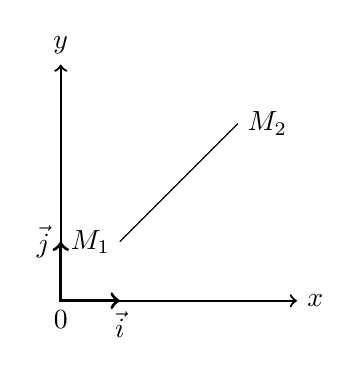
\begin{tikzpicture}[scale=1.5]
      % Draw origin
      \node (0,0) [below] {$0$};
      % Draw axes
      \draw [<->,thick] (0,2) node (yaxis) [above] {$y$}
      |- (2,0) node (xaxis) [right] {$x$};
      % Draw axes
      \draw [<->,very thick] (0,0.5) node (yaxis) [left] {$\vec{j}$}
      |- (0.5,0) node (xaxis) [below] {$\vec{i}$};
      % Draw the segment
      \draw (0.5,0.5) node (M1) [left] {$M_1$} -- (1.5,1.5) node (M2) [right] {$M_2$};
    \end{tikzpicture}
  \end{center}
\end{frame}


%%%%%%%%%%%%%%%%%%%%%%%%%%%%%%%%%%%%%%%%%%%%%%%%%%%%%%%
\begin{frame}{Les deux types de graphisme dans le plan II}

  \begin{alertblock}{Le graphisme POLAIRE (local)}
    Aucune notion de coordonnées.
  \end{alertblock}

  \begin{block}{Deux opérations essentielles}
    \begin{itemize}
    \item \alert{Tourner} à droite ou à gauche sur place d'un angle $a$.
    \item \alert{Avancer} dans la direction courante d'une distance $d$.
    \end{itemize}
  \end{block}

\begin{columns}[c]
  \begin{column}{0.48\textwidth}
    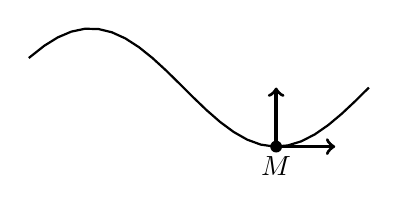
\begin{tikzpicture}[scale=0.75]
    % Draw the curve
    \draw[thick] (pi/6,0.5) -- plot [domain=0.25*pi:2*pi] (\x,{sin(\x r)});
    % Draw the turtle
    \fill (1.5*pi, -1) circle (0.1) node (M) [below] {$M$};
    \draw [->,very thick] (1.5*pi, -1)  -- (1.5*pi+1,-1);
    \draw [->,very thick] (1.5*pi, -1)  -- (1.5*pi,0) ;
  \end{tikzpicture}
  \end{column}
  \begin{column}{0.48\textwidth}
    L'animal traceur porte un repère mobile orthonormé avec une notion de droite et de gauche.
    \\ \alert{la tortue va tourner à gauche}
\end{column}
\end{columns}

\begin{itemize}
\item Opérateurs de translation et de rotation plane, qui engendrent le
groupe des déplacements. La tortue se déplace dans le plan !
\item Graphisme moins matheux, plus intuitif. Inutile de calculer les
coordonnées des points \dots
\item Une trajectoire qui semble lisse sera en fait un polygone !
\end{itemize}
\end{frame}

%%%%%%%%%%%%%%%%%%%%%%%%%%%%%%%%%%%%%%%%%%%%%%%%%%%%%%%
\begin{frame}[fragile]{Le module TurtleGraphics de R}

  Le \alert{graphisme de la tortue} a été inventé au Laboratoire d'Intelligence Artificielle du MIT vers 1968 avec le langage LOGO.
  \begin{itemize}
  \item Il est disponible dans quasiment tous les langages de programmation qui offrent des facilités graphiques.
  \item Et en particulier en R avec le module \alert{TurtleGraphics}.
  \end{itemize}

  \begin{block}{Installation et chargement}
    Ce module n’est pas livré avec la distribution R standard.
    \begin{lstlisting}
install.packages("TurtleGraphics")
\end{lstlisting}


Il faut en importer les noms pour pouvoir les utiliser.
    \begin{lstlisting}
library(TurtleGraphics)
\end{lstlisting}
\end{block}

\end{frame}


%%%%%%%%%%%%%%%%%%%%%%%%%%%%%%%%%%%%%%%%%%%%%%%%%%%%%%%
\begin{frame}{Graphisme cartésien}

  C'est celui des matheux dans la mesure où il faut calculer les coordonnées des points à relier.

  \begin{block}{Représentation de la tortue}
    \begin{itemize}
    \item une flèche qui indique son \alert{cap} en degrés ;
    \item une \alert{position} : une abscisse et une ordonnée ;
    \item un \alert{crayon} (\emph{pen}) qui peut être baissé (\emph{down}) ou levé (\emph{up}).
      Si le crayon est baissé, la tortue laisse une trace en se déplaçant.
      On peut choisir la couleur du crayon ainsi que le type et l’épaisseur de la ligne.
  \end{itemize}
\end{block}

\begin{center}
    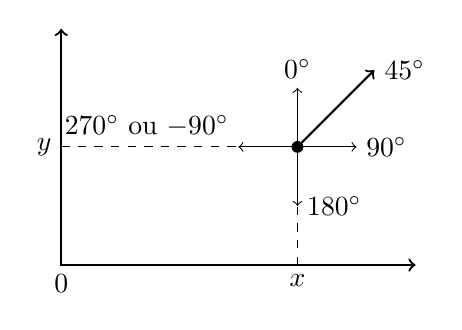
\begin{tikzpicture}[scale=1.5]
      % Draw origin
      \node (0,0) [below] {$0$};
      % Draw axes
      \draw [<->,thick] (0,2) |- (3,0);
      % Draw mobile
      \draw [<->] (2,1.5) node [above] {$0^\circ$}
      |- (2.5,1) node [right] {$90^\circ$};
      \draw [<->] (2,0.5) node [right] {$180^\circ$}
      |- (1.5,1) node [above left] {$270^\circ$ ou $-90^\circ$};
      % Draw the point
      \fill (2, 1) circle (0.05);
      % Draw the vector
      \draw[->,thick] (2, 1) -- (2.65,1.65) node [right] {$45^\circ$};
      % Draw the coordinates
      \draw[dashed] (2, 0) node [below] {$x$} -- (2,1);
      \draw[dashed] (0, 1) node [left] {$y$} -- (2,1);
    \end{tikzpicture}
  \end{center}
\end{frame}

%%%%%%%%%%%%%%%%%%%%%%%%%%%%%%%%%%%%%%%%%%%%%%%%%%%%%%%
\begin{frame}[fragile]{État et opération de la tortue}
  Une tortue a donc un ETAT représenté mathématiquement par trois données : position ; cap ; crayon.


\begin{columns}[t]
\begin{column}{0.48\textwidth}
  \begin{block}{Position}
    \begin{lstlisting}[style=edblock]
turtle_getpos()
turtle_setpos(x,y)
\end{lstlisting}
  \end{block}

\begin{block}{Crayon (état)}
    \begin{lstlisting}[style=edblock]
turtle_down()
turtle_up()
\end{lstlisting}
\end{block}

\begin{alertblock}{Tracer un segment}
    \begin{lstlisting}[style=edblock]
turtle_goto(x, y)
\end{lstlisting}
\end{alertblock}

\end{column}
\begin{column}{0.48\textwidth}
  \begin{block}{Cap}
    \begin{lstlisting}[style=edblock]
turtle_getangle()
turtle_setangle(a)
    \end{lstlisting}
  \end{block}

\begin{block}{Crayon (style)}
    \begin{lstlisting}[style=edblock]
turtle_param(col, lwd ,lty)
turtle_col(col)
turtle_lwd(lwd)
turtle_lty(lty)
\end{lstlisting}
\end{block}
\end{column}
\end{columns}

\end{frame}

%%%%%%%%%%%%%%%%%%%%%%%%%%%%%%%%%%%%%%%%%%%%%%%%%%%%%%%
\begin{frame}[fragile]{Dessin d'un triangle rectangle}

  \begin{block}{Agir sur le bac à sable (canevas)}
    \begin{lstlisting}[style=edblock]
turtle_init(width = 100, height = 100,
            mode = c("error", "clip", "cycle"))
turtle_reset()
\end{lstlisting}


\begin{columns}[c]
\begin{column}{0.63\textwidth}
  \begin{lstlisting}[style=editor]
TriRect <- function(a, b, c = 10) {
  turtle_up()
  turtle_goto(c, c);
  turtle_down()
  turtle_goto(a + c, c)
  turtle_goto(c, b + c)
  turtle_goto(c, c)
}
\end{lstlisting}

\begin{lstlisting}[linerange=2-3]
png("fig/trirect.png")
turtle_init(width = 100, height = 70)
turtle_do(TriRect(80, 50))
dev.off()
\end{lstlisting}
\end{column}
\begin{column}{0.35\textwidth}
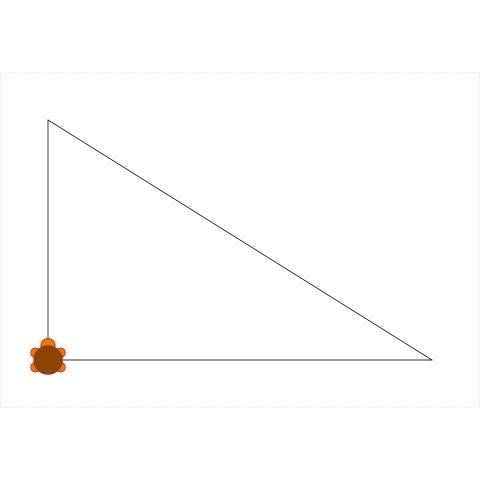
\includegraphics[width=4cm]{trirect}
\end{column}
\end{columns}
  \end{block}

  \alert{ATTENTION}, les points du canevas ont des coordonnées positives. \\
  L'origine du repère est donc en bas à gauche.
\end{frame}


%%%%%%%%%%%%%%%%%%%%%%%%%%%%%%%%%%%%%%%%%%%%%%%%%%%%%%%
\begin{frame}[fragile]{Tracé de la courbe du cosinus}

\begin{columns}[c]
\begin{column}{0.63\textwidth}
\begin{lstlisting}[style=editor]
TraceFunction <- function(f, a, b, n) {
  turtle_up()
  turtle_goto(a, f(a))
  turtle_down()
  for(x in seq(a,b, length.out=n)) {
    turtle_goto(x, f(x))
  }
}
\end{lstlisting}

\begin{lstlisting}[linerange=2-6]
png("fig/cos.png")
b <- 50
n <- 1000
turtle_init(width= b, height= b)
f <- function(x) b * (cos(x)+1) / 2
turtle_do(TraceFunction(f, 0, b, n))
dev.off()
\end{lstlisting}
\end{column}
\begin{column}{0.35\textwidth}
 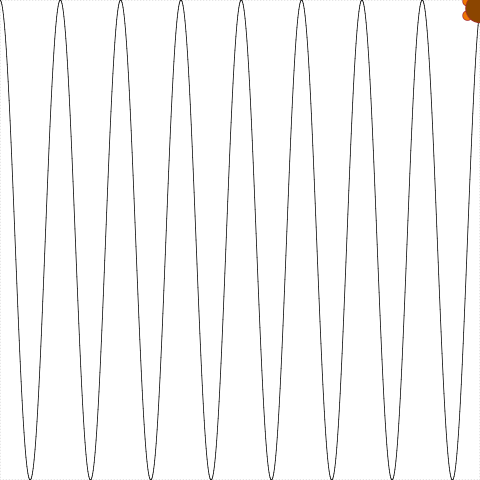
\includegraphics[width=4cm]{cos}
\end{column}
\end{columns}

Comme \texttt{turtle\_goto} ou \texttt{TraceFunction} , la plupart des fonctions de dessin n'ont \alert{pas de résultat, seulement des effets}.
\end{frame}

%%%%%%%%%%%%%%%%%%%%%%%%%%%%%%%%%%%%%%%%%%%%%%%%%%%%%%%
\begin{frame}{Courbes en coordonnées paramétriques}

\end{frame}

%%%%%%%%%%%%%%%%%%%%%%%%%%%%%%%%%%%%%%%%%%%%%%%%%%%%%%%
\questionSlide

%%%%%%%%%%%%%%%%%%%%%%%%%%%%%%%%%%%%%%%%%%%%%%%%%%%%%%%
 \appendix
 \backupSlides
%%%%%%%%%%%%%%%%%%%%%%%%%%%%%%%%%%%%%%%%%%%%%%%%%%%%%%%

%%%%%%%%%%%%%%%%%%%%%%%%%%%%%%%%%%%%%%%%%%%%%%%%%%%%%%%
% \begin{frame}[fragile]{Backup slides}
%   Sometimes, it is useful to add slides at the end of your presentation to
%   refer to during audience questions.

%   The best way to do this is to include the \verb|appendixnumberbeamer|
%   package in your preamble and call \verb|\appendix| before your backup slides.

%   will automatically turn off slide numbering and progress bars for
%   slides in the appendix.
% \end{frame}


%%%%%%%%%%%%%%%%%%%%%%%%%%%%%%%%%%%%%%%%%%%%%%%%%%%%%%%
% \begin{frame}[allowframebreaks]{References}

%   % \bibliography{../bib_parallelism,../bib_others}
%   % \bibliographystyle{abbrv}

% \end{frame}

\end{document}

%%% Local Variables:
%%% mode: latex
%%% TeX-master: t
%%% End:
